\subsection{Introducción}

El ESP32 es el microcontrolador principal del proyecto, y se encuentra instalado en la motherboard. Las señales utilizadas por el hardware del proyecto son medidas por los sensores de la motherboard y procesadas por el microcontrolador. A su vez, el microcontrolador se encarga de controlar y operar el hardware. La ESP32, además de ser el núcleo “lógico” del sistema, también es el nexo entre los componentes analógicos (principalmente sensores) y la página web, que recibirá, continuará procesando, y mostrará los datos enviados por el microcontrolador, únicos para cada usuario.\\

Este ESP32 es programada en micropython, que es una implementación del lenguaje Python especializada en microcontroladores. Decidimos utilizar Python al ser un lenguaje de alto nivel, con gran amplitud de librerías estándar que facilitan su implementación, convirtiéndolo en un lenguaje sencillo de programar. Aunque, a comparación de c, los programas hechos en python son más lentos, la velocidad de ejecución no representará un obstáculo al funcionamiento correcto del sistema, ya que los procesos que requieren de una rápida ejecución (en este caso, la lógica del cargador MPPT) serán ejecutados sobre las Raspberry Pi Pico, los microcontroladores secundarios del proyecto.\\

El hardware de la motherboard mide los siguientes datos:

\begin{itemize}
    \item Voltaje de la red del proveedor.
    \item Voltaje de batería.
    \item Cruce por cero.
\end{itemize}
Además, recibirá la medición de corriente de cada línea de los sensores de corriente externos.\\

A partir de estos datos, el microcontrolador procesa y calcula la siguiente información:
\begin{itemize}
    \item Promedio de tensión de la red del proveedor.
    \item Picos de corriente de las líneas.
    \item Consumo de cada línea.
\end{itemize}

Con esta información, el microcontrolador hace dos cosas: por un lado, envía la información al servidor de la página web a través de un método POST; el servidor calcula nuevos datos mediante la información recibida, y almacena todo en la base de datos del servidor. Por otro lado, controla el conmutador en base a parámetros definidos: comparando los consumos de la línea con un valor de umbral consumo. Si el consumo medido es inferior al valor de umbral, el microcontrolador acciona el conmutador para que conmute la fuente de la línea a la fuente de energía solar. Si el consumo medido fuese superior al valor de umbral, se conmutará la línea a la red del proveedor eléctrico.\\

Por último, el ESP32 enviará un pulso a la Pi Pico, y ésta le devolverá la información del promedio de consumo en una hora y voltaje de la batería. La comunicación entre ambos microcontroladores se realiza utilizando el protocolo UART; la ESP32 es el microcontrolador master mientras que la Raspberry Pi Pico es el microcontrolador slave.\\ 

La información recibida de parte de la Raspberry Pi Pico también será enviada al servidor web para mostrar al usuario, mientras que la información del voltaje de la batería inhibirá al conmutador de las líneas eléctricas del sistema en caso de ser demasiado baja.\\


\subsection{Librería SolarLink}

La librería “solarlink.py” contiene todas las funciones necesarias para medir la señal de los sensores y manejar los datos del sistema. El programa principal utiliza esta librería para ejecutar tareas específicas. Todo el código base se encuentra en la librería principal del programa para evitar redundancias y para mantener limpio el código del programa principal. Actualmente, la librería consiste de la clase SolarLink.

\subsubsection{Clase SolarLink}

La clase SolarLink contiene las funciones 
\mint{python}|def __init__(self)| 
\mint{python}|def callback_fin_mediciones(self, t)|
\mint{python}|def corriente_dif_read(self, pin a, pin b)|
\mint{python}|def voltaje_read(self)|
\mint{python}|def medicion_default_segundo()|

La función \textbf{init} es el constructor de la librería, que se encarga de configurar e inicializar los ADC interno y externo, el protocolo I2C que habilita la comunicación con el ADC externo; y definir el valor de la pendiente de la corriente en función de la tensión, la referencia del sensor de voltaje, los atributos del Timer, el Callback del timer, y la medición final. Se puede ver su implementación en Listing \ref{main-1} y Listing \ref{main-2}\\

El método \textbf{callback\_fin\_mediciones} tiene como única función setear el atributo \textbf{self.fin\_mediciones} cada vez que se ejecuta el callback del timer, que actúa como flag (Listing \ref{callback-mediciones}).\\

El método \textbf{corriente\_dif\_read} se encarga de obtener la diferencia de voltaje entre los dos pines del ADC externo, al cual le corresponderá cada sensor respectivamente. La diferencia de voltaje es multiplicada por el valor de la pendiente de la corriente en función de la tensión, y dividido por la raíz de dos, obteniendo así el valor de corriente eficaz que luego es devuelto por el método (Listing \ref{clase corriente}).\\

El método \textbf{voltaje\_read} se encarga de medir en microvolts la señal otorgada por el sensor de voltaje, que corresponderá a un valor de tensión eficaz. Luego, este valor se traspasa a volts y se lo multiplica por el valor de referencia del sensor de tensión, así obteniendo el valor equivalente de la tensión de línea. Este dato será la variable devuelta por el método (Listing \ref{clase voltaje}).\\

El método \textbf{medicion\_default\_segundo} realiza múltiples mediciones en un periodo de 1 segundo. El valor devuelto por este método es el dato principal que utilizará el programa main a la hora de realizar tareas específicas (Listing \ref{medicion default segundo}).\\

El bucle principal de la clase se ejecuta de manera constante, y empieza sumando múltiples mediciones de voltaje llamando a \textbf{voltaje\_read}, para promediar el valor posteriormente (Listing \ref{bucle main}).\\

Luego se procede a obtener las mediciones de los dos sensores de corriente, llamando a la función \textbf{corriente\_dif\_read}. Dos bucles if evalúan si la corriente medida es mayor al último pico de corriente registrado, y si no lo es, guarda el valor medido en la variable de pico de corriente, almacenando así los picos máximos de corriente históricos.\\

Un bucle if evalúa la condición del callback del timer. Al pasar un segundo, el callback se setea y se ejecuta el código dentro del bucle. Primero, se saca el promedio de la suma de mediciones de voltaje obtenidas al comienzo del bucle principal de la clase, y se asigna los picos de las dos líneas utilizadas a las variables de valor de corriente respectivos. Se obtiene el consumo de cada línea multiplicando el voltaje promedio por el valor de corriente de cada línea.\\

El \textbf{atributo self.medicion} almacena el valor de voltaje promedio, las corrientes de cada línea, y los consumos de cada línea.\\

Se reinician las variables de picos de corriente, la suma de voltajes, el índice de la suma, y el callback del timer. Finalmente, se rompe el bucle y se retorna el atributo \textbf{self.medicion}.


\subsection{Programa principal}

El programa principal main.py realiza tareas específicas, como el muestreo de datos básicos al display LCD que se encuentra conectado al microcontrolador, el control del conmutador de líneas, y el posteo de los datos al servidor web de SolarLink, que se realiza utilizando las librerías microdot y requests. El programa utiliza la librería SolarLink para obtener los valores de mediciones, llamando a la clase dentro del código principal. Fuera del bucle principal, también se define los pines a los que irán conectados el conmutador, que luego será activado dentro del bucle.

\subsubsection{Bucle principal}

El bucle principal trabaja con los valores devueltos por el método \textbf{medicion\_default\_segundo} de la clase SolarLink. Un display LCD se encarga de mostrar todos los datos devueltos por el método.\\

El diccionario con los valores es convertido a las variables \textit{voltaje}, \textit{corriente\_l1}, \textit{corriente\_l2}, \textit{consumo\_l1}, y \textit{consumo\_l2}. Luego, se colocan en off los pines p\_l1 y p\_l2, que corresponden a los del conmutador. Finalmente, se establece una variable en 100. Esta variable será el threshold de consumo que determinará si se activa el conmutador o no.\\

Un condicional revisa si la suma de la suma de los consumos de ambas líneas es menor al trigger. De ser el caso, conmutará ambas líneas a la red solar. Caso contrario, revisará si el consumo de la primer línea o si el de la segunda es inferior al trigger, y entonces conmutará la línea correspondiente a la red solar. Si ambos consumos son mayores al valor del trigger, entonces conmutará ambas líneas a la red del proveedor.

\subsubsection{Microdot y posteo de datos}

Microdot se encargará de ayudar a decidir a qué usuario le corresponde el módulo Solar Link. Esta pestaña será de visualización sencilla, para no sobrecargar al microcontrolador.

\begin{figure}[H]
    \centering
    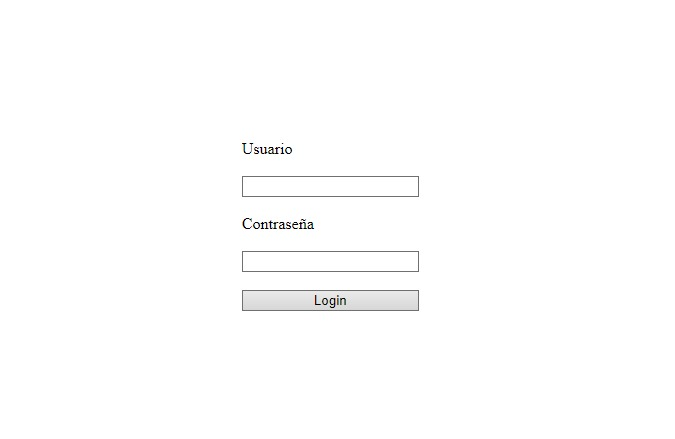
\includegraphics[width=1\linewidth]{WhatsApp Image 2023-10-16 at 21.25.50.jpeg}
    \caption{Página de configuración del micro.}
    \label{fig:enter-label}
\end{figure}

